
%%% Local Variables:
%%% mode: latex
%%% TeX-master: "main"
%%% End:
\chapter{Rutherford's Alpha Particle Scattering Experiment}

\begin{figure}[H]
  \centering
  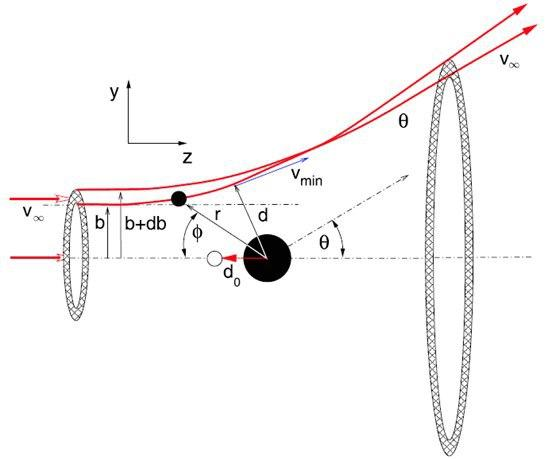
\includegraphics[width=0.5\linewidth]{figures/Rutherford}
  \label{fig:}
\end{figure}

According to Columb's Law:

\begin{equation*}
  \begin{aligned}
    F = \dfrac{1}{4 \pi \varepsilon_0} \cdot \dfrac{Z_1 Z_2 e^2}{r^2} = \dfrac{C}{r^2}
  \end{aligned}
\end{equation*}
\begin{equation*}
  \begin{aligned}
    C = \dfrac{Z_1 Z_2 e^2}{4 \pi \varepsilon_0} 
  \end{aligned}
\end{equation*}
\begin{equation*}
  \begin{aligned}
    F_y = F \sin \phi = \dfrac{C}{r^2} \sin \phi 
  \end{aligned}
\end{equation*}

Law of momentum and angular momentum
\begin{equation*}
  \begin{aligned}
    m v_y = \int F_y \md t
  \end{aligned}
\end{equation*}
\begin{equation*}
  \begin{aligned}
    m r^2 \dot{\phi} = m v_{\infty} b
  \end{aligned}
\end{equation*}

Then we integrate

\begin{equation*}
  \begin{aligned}
    v_y &= \dfrac{1}{m} \int \dfrac{C}{r^2} \sin \phi \md t
    = \dfrac{1}{m} \int \dfrac{C}{r^2} \sin \phi \dfrac{\md t}{\md \phi} \md \phi 
    = \dfrac{1}{m} \int \dfrac{C}{r^2} \sin \phi \dfrac{r^2}{v_{\infty} b}  \md \phi
    = \dfrac{C}{m v_{\infty} b} \int_0^{\pi - \theta} \sin \phi \md \phi\\
    &= \dfrac{C}{m v_{\infty} b} \left( 1 + \cos \theta \right) 
  \end{aligned}
\end{equation*}

Now we need to relate $\theta$ with $b$, Since

\begin{equation*}
  \begin{aligned}
    v_y = v_\infty \sin \theta
  \end{aligned}
\end{equation*}

We have

\begin{equation*}
  \begin{aligned}
    \dfrac{C}{m v_{\infty} b} \left( 1 + \cos \theta \right) = v_{\infty} \sin \theta
  \end{aligned}
\end{equation*}

So that

\begin{equation*}
  \begin{aligned}
    \cot \dfrac{\theta}{2} = \dfrac{1 + \cos \theta}{\sin \theta} = \dfrac{m v_{\infty}^2 b}{C} = \dfrac{2 E_0 b}{C} 
  \end{aligned}
\end{equation*}

Note that this trigonometry transform is used

\begin{equation*}
  \begin{aligned}
    \dfrac{1 + \cos \theta}{\sin \theta} = \dfrac{2 \cos^2 \dfrac{\theta}{2}}{2 \sin \dfrac{\theta}{2} \cos \dfrac{\theta}{2}} = \cot \dfrac{\theta}{2}
  \end{aligned}
\end{equation*}

Finally

\begin{equation*}
  \begin{aligned}
    b = \dfrac{C}{2 E_0} \cdot \cot \dfrac{\theta}{2} = \dfrac{1}{4 \pi \varepsilon_0} \dfrac{Z_1 Z_2 e^2}{2 E_0} = \dfrac{1}{4 \pi \varepsilon_0} \cdot \dfrac{Z_1 Z_2 e^2}{m v_{\infty}} \cdot \cot \dfrac{\theta}{2} 
  \end{aligned}
\end{equation*}

Now we begin to find the relation between $\md b$ and $\md \Omega$

\begin{figure}[H]
  \centering
  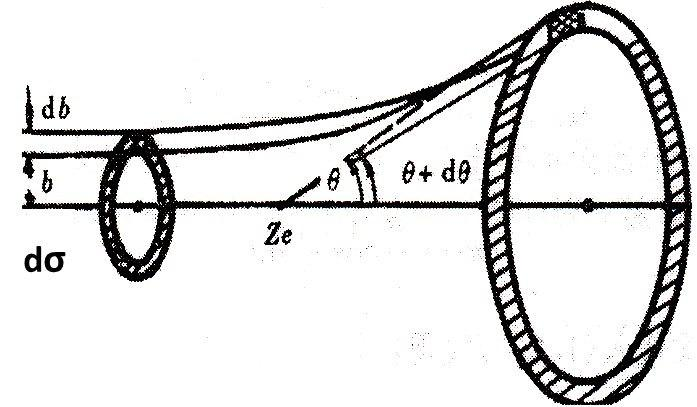
\includegraphics[width=0.5\linewidth]{figures/Rutherford-1}
  \label{fig:}
\end{figure}

\begin{equation*}
  \begin{aligned}
    \md \sigma = 2 \pi b \md b = \pi \left( \dfrac{1}{4 \pi \varepsilon_0}  \right)^2 \left( \dfrac{Z_1 Z_2 e^2}{m v_{\infty}^2}  \right)^2 \dfrac{\cos \dfrac{\theta}{2} }{\sin^3 \dfrac{\theta}{2} } \md \theta 
  \end{aligned}
\end{equation*}
\begin{equation*}
  \begin{aligned}
    \Omega &= 2 \pi \left( 1 - \cos \theta \right) \\
    \md \Omega &= 2 \pi \sin \theta \md \theta = 4 \pi \sin \dfrac{\theta}{2} \cos \dfrac{\theta}{2} \md \theta  
  \end{aligned}
\end{equation*}

Then we found $\dfrac{\md \sigma}{\md \Omega}$ is only related with $\theta$

\begin{equation*}
  \begin{aligned}
    \dfrac{\md \sigma}{\md \Omega} = \left( \dfrac{1}{4 \pi \varepsilon_0}  \right)^2 \left( \dfrac{Z_1 Z_2 e^2}{2 m v_{\infty}^2}  \right)^2 \sin^{-4} \dfrac{\theta}{2}
  \end{aligned}
\end{equation*}

As for a thin gold leaf, we assume there's only one layer of atoms, the density of atoms is $N$, the area and thickness of gold leaf are $A$ and $t$

When $n$ particles passed through the gold leaf, $\md n$ of them ended up in $\md \Omega$

\begin{equation*}
  \begin{aligned}
    \dfrac{\md n}{n} = \dfrac{N A t \md \sigma}{A} = N t \md \sigma = N t \left( \dfrac{1}{4 \pi \varepsilon_0}  \right)^2 \left( \dfrac{Z_1 Z_2 e^2}{2 m v_{\infty}^2}  \right)^2 \sin^{-4} \dfrac{\theta}{2} \md \Omega 
  \end{aligned}
\end{equation*}
\begin{equation*}
  \begin{aligned}
    \dfrac{\md n}{\md \Omega} \sin^4 \dfrac{\theta}{2} = n N t \left( \dfrac{1}{4 \pi \varepsilon_0}  \right)^2 \left( \dfrac{Z_1 Z_2 e^2}{2 m v_{\infty}^2}  \right)^2 = \mathrm{const}
  \end{aligned}
\end{equation*}

For alpha particles, $Z_1 = 2$. We can also take the closest distance between the 2 particles as the radius of a particle.

\begin{figure}[H]
  \centering
  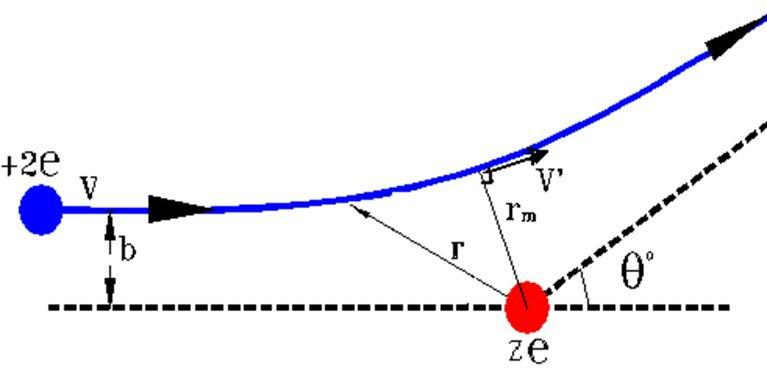
\includegraphics[width=0.5\linewidth]{figures/Rutherford-2}
  \label{fig:}
\end{figure}

What we have already known are:

\begin{equation*}
  \begin{aligned}
    \dfrac{1}{2} M V^2 = \dfrac{1}{2} M V'^{2} + \dfrac{2 Z e^2}{4 \pi \varepsilon_0 r_m}  
  \end{aligned}
\end{equation*}
\begin{equation*}
  \begin{aligned}
    M V b = M V' r_m
  \end{aligned}
\end{equation*}
\begin{equation*}
  \begin{aligned}
    b = \dfrac{1}{4 \pi \varepsilon_0} \cdot \dfrac{2 Z e^2}{M V}} \cdot \cot \dfrac{\theta}{2} 
  \end{aligned}
\end{equation*}

We solve $r_m$ with the equation we known.

\begin{equation*}
  \begin{aligned}
    \dfrac{1}{4 \pi \varepsilon_0} \cdot \dfrac{2 Z e^2}{M}} \cdot \cot \dfrac{\theta}{2} = V' r_m
  \end{aligned}
\end{equation*}

\begin{equation*}
  \begin{aligned}
    \dfrac{1}{2} M V^2 = \dfrac{1}{2} M \left( \dfrac{1}{4 \pi \varepsilon_0} \cdot \dfrac{2 Z e^2}{M r_m}} \cdot \cot \dfrac{\theta}{2} \right)^{2} + \dfrac{2 Z e^2}{4 \pi \varepsilon_0 r_m}  
  \end{aligned}
\end{equation*}

\begin{equation*}
  \begin{aligned}
    \dfrac{1}{2} M V^2 r_m^2 - \dfrac{2 Z e^2}{4 \pi \varepsilon_0} r_m - \dfrac{1}{2} M \left( \dfrac{1}{4 \pi \varepsilon_0} \cdot \dfrac{2 Z e^2}{M}} \cdot \cot \dfrac{\theta}{2} \right)^{2} = 0
  \end{aligned}
\end{equation*}

Finally

\begin{equation*}
  \begin{aligned}
    r_m = \dfrac{1}{4 \pi \varepsilon_0} \dfrac{2 z e^2}{M V^2} \left( 1 + \dfrac{1}{\sin \dfrac{\theta}{2} }  \right)  
  \end{aligned}
\end{equation*}

